% LaTeX: Visual Workflow and Conceptual Diagrams
% Requires: \usepackage{tikz}, \usepackage{pgfplots}

\section{Visual Workflow Representation}
\label{sec:visual-workflow}

\subsection{Overall System Architecture}

\begin{figure}[h]
\centering
\begin{tikzpicture}[
    node distance=1.5cm,
    box/.style={rectangle, draw, thick, text width=3cm, text centered, minimum height=1cm, fill=blue!10},
    data/.style={cylinder, draw, thick, text width=2.5cm, text centered, minimum height=0.8cm, fill=green!10, aspect=0.3},
    arrow/.style={->, thick, >=stealth}
]

% Data sources
\node[data] (repos) {JavaScript Repositories};
\node[data, below=of repos] (smells_db) {Study Smells Database};

% Processing layers
\node[box, right=3cm of repos] (detection) {Smell Detection\\(Steel + SNutsJS)};
\node[box, below=of detection] (refactor) {LLM Refactoring\\(Multi-Strategy)};
\node[box, below=of refactor] (execution) {Test Execution\\+ Validation};

% Output
\node[data, right=3cm of refactor] (experiments) {Experiments Database};
\node[box, above=0.5cm of experiments] (analysis) {Statistical Analysis};

% Arrows
\draw[arrow] (repos) -- (detection);
\draw[arrow] (detection) -- (smells_db);
\draw[arrow] (smells_db) -- (refactor);
\draw[arrow] (refactor) -- (execution);
\draw[arrow] (execution) -- (experiments);
\draw[arrow] (experiments) -- (analysis);

% Labels
\node[above=0.2cm of detection, font=\small\itshape] {Baseline};
\node[above=0.2cm of refactor, font=\small\itshape] {Phase 1};
\node[above=0.2cm of execution, font=\small\itshape] {Phase 2};

\end{tikzpicture}
\caption{High-Level System Architecture}
\label{fig:architecture}
\end{figure}

\subsection{Two-Phase Experiment Workflow}

\begin{figure}[h]
\centering
\begin{tikzpicture}[
    node distance=0.8cm,
    step/.style={rectangle, draw, thick, text width=4cm, text centered, minimum height=0.8cm, fill=orange!20},
    decision/.style={diamond, draw, thick, text width=2.5cm, text centered, aspect=2, fill=yellow!20},
    phase/.style={rectangle, draw, ultra thick, dashed, text width=10cm, minimum height=6cm},
    arrow/.style={->, thick, >=stealth}
]

% Phase 1 Box
\node[phase, label=above left:\textbf{PHASE 1: REFACTORING}] (p1box) at (0,0) {};

\node[step] (p1s1) at (0, 2) {Load Smell Context};
\node[step, below=of p1s1] (p1s2) {Build Prompt (Strategy)};
\node[step, below=of p1s2] (p1s3) {Call LLM API};
\node[step, below=of p1s3] (p1s4) {Extract Code};
\node[step, below=of p1s4] (p1s5) {Save to Database};

% Phase 2 Box
\node[phase, label=above left:\textbf{PHASE 2: EXECUTION}, below=3cm of p1box] (p2box) {};

\node[step] (p2s1) at (0, -6) {Load Refactored Code};
\node[step, below=of p2s1] (p2s2) {Backup + Apply};
\node[step, below=of p2s2] (p2s3) {Run Smell Detection};
\node[step, below=of p2s3] (p2s4) {Run Test Suite};
\node[step, below=of p2s4] (p2s5) {Analyze Results};
\node[step, below=of p2s5] (p2s6) {Restore Backup};

% Arrows Phase 1
\draw[arrow] (p1s1) -- (p1s2);
\draw[arrow] (p1s2) -- (p1s3);
\draw[arrow] (p1s3) -- (p1s4);
\draw[arrow] (p1s4) -- (p1s5);

% Connection between phases
\draw[arrow, ultra thick, blue] (p1s5) -- node[right, text width=3cm] {Manifest File or Query} (p2s1);

% Arrows Phase 2
\draw[arrow] (p2s1) -- (p2s2);
\draw[arrow] (p2s2) -- (p2s3);
\draw[arrow] (p2s3) -- (p2s4);
\draw[arrow] (p2s4) -- (p2s5);
\draw[arrow] (p2s5) -- (p2s6);

\end{tikzpicture}
\caption{Two-Phase Experiment Workflow}
\label{fig:two-phase}
\end{figure}

\subsection{Prompt Strategy Comparison}

\begin{figure}[h]
\centering
\begin{tikzpicture}[
    node distance=1.2cm,
    component/.style={rectangle, draw, thick, text width=2.8cm, minimum height=0.6cm, text centered, font=\small},
    arrow/.style={->, thick, >=stealth}
]

% Zero-Shot
\node[component, fill=red!20] (zs_title) at (0, 4) {\textbf{Zero-Shot}};
\node[component, below=0.3cm of zs_title] (zs1) {Task Definition};
\node[component, below=0.2cm of zs1] (zs2) {Smell Definition};
\node[component, below=0.2cm of zs2] (zs3) {Original Code};
\node[component, below=0.2cm of zs3] (zs4) {Output Constraints};
\node[below=0.2cm of zs4, font=\tiny] (zs_size) {$\sim$200 tokens};

% Few-Shot
\node[component, fill=green!20] (fs_title) at (4, 4) {\textbf{Few-Shot}};
\node[component, below=0.3cm of fs_title] (fs1) {Task Definition};
\node[component, below=0.2cm of fs1] (fs2) {Smell Definition};
\node[component, below=0.2cm of fs2, fill=green!40] (fs3) {1-3 Examples};
\node[component, below=0.2cm of fs3] (fs4) {Original Code};
\node[component, below=0.2cm of fs4] (fs5) {Output Constraints};
\node[below=0.2cm of fs5, font=\tiny] (fs_size) {$\sim$600 tokens};

% Chain-of-Thought
\node[component, fill=blue!20] (cot_title) at (8, 4) {\textbf{Chain-of-Thought}};
\node[component, below=0.3cm of cot_title] (cot1) {Task Definition};
\node[component, below=0.2cm of cot1] (cot2) {Smell Definition};
\node[component, below=0.2cm of cot2, fill=blue!40] (cot3) {Detection Criteria};
\node[component, below=0.2cm of cot3, fill=blue!40] (cot4) {Refactor Strategies};
\node[component, below=0.2cm of cot4] (cot5) {0-2 Examples};
\node[component, below=0.2cm of cot5] (cot6) {Original Code};
\node[component, below=0.2cm of cot6, fill=blue!40] (cot7) {CoT Template};
\node[component, below=0.2cm of cot7] (cot8) {Output Constraints};
\node[below=0.2cm of cot8, font=\tiny] (cot_size) {$\sim$800 tokens};

% Comparison labels
\node[rotate=90, above left=0.5cm and -0.5cm of zs_title] {\small Complexity $\rightarrow$};

\end{tikzpicture}
\caption{Prompt Strategy Components Comparison}
\label{fig:prompt-strategies}
\end{figure}

\subsection{LLM Provider Distribution}

\begin{figure}[h]
\centering
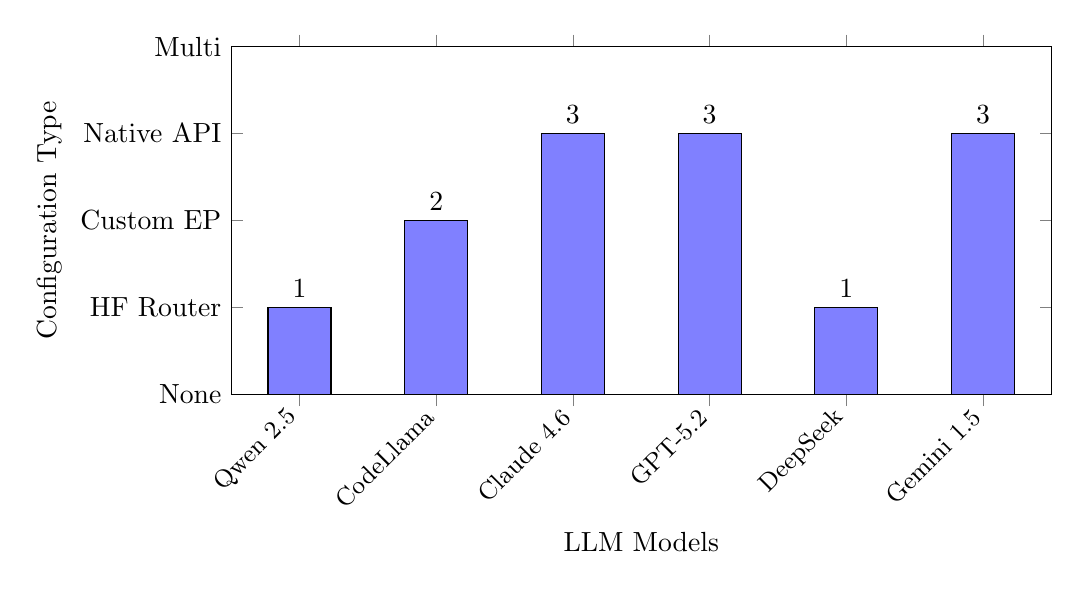
\begin{tikzpicture}
\begin{axis}[
    ybar,
    bar width=0.8cm,
    width=12cm,
    height=6cm,
    xlabel={LLM Models},
    ylabel={Configuration Type},
    symbolic x coords={Qwen 2.5, CodeLlama, Claude 4.6, GPT-5.2, DeepSeek, Gemini 1.5},
    xtick=data,
    x tick label style={rotate=45, anchor=east, font=\small},
    ymin=0, ymax=4,
    ytick={0,1,2,3,4},
    yticklabels={None, HF Router, Custom EP, Native API, Multi},
    legend pos=north west,
    nodes near coords,
]

\addplot[fill=blue!50] coordinates {
    (Qwen 2.5, 1)
    (CodeLlama, 2)
    (Claude 4.6, 3)
    (GPT-5.2, 3)
    (DeepSeek, 1)
    (Gemini 1.5, 3)
};

\end{axis}
\end{tikzpicture}
\caption{LLM Provider API Configuration Types}
\label{fig:providers}
\end{figure}

\subsection{Experiment State Machine}

\begin{figure}[h]
\centering
\begin{tikzpicture}[
    node distance=2.5cm,
    state/.style={circle, draw, thick, minimum size=1.5cm, text centered, font=\small},
    arrow/.style={->, thick, >=stealth}
]

% States
\node[state, fill=gray!20] (created) {Created};
\node[state, fill=yellow!20, right=of created] (refactored) {Refactored};
\node[state, fill=green!20, right=of refactored] (executed) {Executed};
\node[state, fill=red!20, below=1cm of refactored] (failed) {Failed};

% Transitions
\draw[arrow] (created) -- node[above, font=\scriptsize] {Phase 1 Success} (refactored);
\draw[arrow] (refactored) -- node[above, font=\scriptsize] {Phase 2 Success} (executed);
\draw[arrow] (created) -- node[left, font=\scriptsize] {LLM Error} (failed);
\draw[arrow] (refactored) -- node[right, font=\scriptsize] {Test Failure} (failed);
\draw[arrow] (executed) to[bend left=60] node[below, font=\scriptsize] {--redo flag} (refactored);

% Flags
\node[below=0.3cm of created, font=\tiny, text width=2cm, text centered] {refactor\_phase = F\\execution\_phase = F};
\node[below=0.3cm of refactored, font=\tiny, text width=2cm, text centered] {refactor\_phase = T\\execution\_phase = F};
\node[below=0.3cm of executed, font=\tiny, text width=2cm, text centered] {refactor\_phase = T\\execution\_phase = T};

\end{tikzpicture}
\caption{Experiment Lifecycle State Machine}
\label{fig:state-machine}
\end{figure}

\subsection{Database Entity Relationship}

\begin{figure}[h]
\centering
\begin{tikzpicture}[
    entity/.style={rectangle, draw, thick, text width=3cm, text centered, minimum height=1cm, fill=blue!10},
    relationship/.style={diamond, draw, thick, text width=1.5cm, text centered, aspect=2, fill=yellow!10},
    arrow/.style={-, thick}
]

% Entities
\node[entity] (repo) {Repository};
\node[entity, below right=2cm and 2cm of repo] (file) {File};
\node[entity, below left=2cm and 2cm of file] (smell) {StudySmells};
\node[entity, right=3cm of file] (exp) {Experiment};
\node[entity, above right=1cm and 1cm of exp] (testres) {TestResult};
\node[entity, below right=1cm and 1cm of exp] (smellres) {SmellResult};

% Relationships
\draw[arrow] (repo) -- (file);
\draw[arrow] (file) -- (smell);
\draw[arrow] (smell) -- (exp);
\draw[arrow] (file) -- (exp);
\draw[arrow] (exp) -- (testres);
\draw[arrow] (exp) -- (smellres);

% Cardinalities
\node[above=0.2cm of file, anchor=south west, font=\tiny] {1:N};
\node[above=0.2cm of smell, anchor=south east, font=\tiny] {1:N};
\node[above=0.2cm of exp, anchor=south west, font=\tiny] {1:N};
\node[right=0.1cm of testres, anchor=west, font=\tiny] {1:N};
\node[right=0.1cm of smellres, anchor=west, font=\tiny] {1:N};

\end{tikzpicture}
\caption{Simplified Database Entity-Relationship Diagram}
\label{fig:er-diagram}
\end{figure}

\subsection{Validation Metrics Hierarchy}

\begin{figure}[h]
\centering
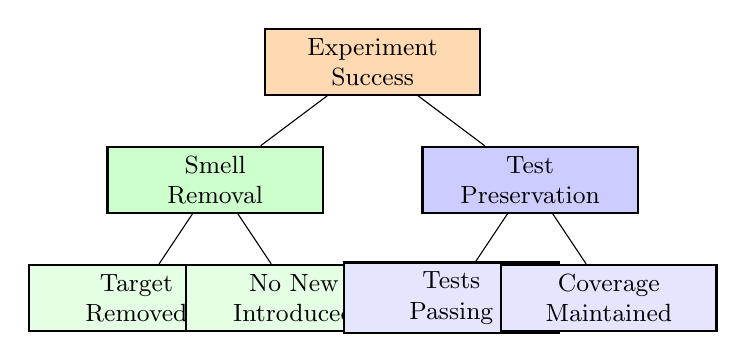
\begin{tikzpicture}[
    level 1/.style={sibling distance=4cm, level distance=1.5cm},
    level 2/.style={sibling distance=2cm, level distance=1.5cm},
    metric/.style={rectangle, draw, thick, text width=2.5cm, text centered, minimum height=0.7cm, font=\small},
]

\node[metric, fill=orange!30] {Experiment\\Success}
    child { node[metric, fill=green!20] {Smell\\Removal}
        child { node[metric, fill=green!10] {Target\\Removed} }
        child { node[metric, fill=green!10] {No New\\Introduced} }
    }
    child { node[metric, fill=blue!20] {Test\\Preservation}
        child { node[metric, fill=blue!10] {Tests\\Passing} }
        child { node[metric, fill=blue!10] {Coverage\\Maintained} }
    };

\end{tikzpicture}
\caption{Hierarchical Validation Metrics}
\label{fig:metrics}
\end{figure}

\subsection{Batch Processing Flow}

\begin{figure}[h]
\centering
\begin{tikzpicture}[
    node distance=1cm,
    box/.style={rectangle, draw, thick, text width=3cm, text centered, minimum height=0.7cm, font=\small},
    decision/.style={diamond, draw, thick, text width=2cm, text centered, aspect=2, font=\small},
    arrow/.style={->, thick, >=stealth}
]

\node[box, fill=blue!20] (start) {Load Smell List};
\node[box, below=of start] (filter) {Apply Filters\\(limit, start-from)};
\node[decision, below=of filter] (check) {More\\Smells?};
\node[box, right=2cm of check] (process) {Process Smell};
\node[decision, below=of process] (success) {Success?};
\node[box, left=2cm of success] (record) {Record Statistics};
\node[box, below=2cm of check] (summary) {Generate\\Summary};

% Main flow
\draw[arrow] (start) -- (filter);
\draw[arrow] (filter) -- (check);
\draw[arrow] (check) -- node[above, font=\tiny] {Yes} (process);
\draw[arrow] (process) -- (success);
\draw[arrow] (success) -- node[above, font=\tiny] {Yes/No} (record);
\draw[arrow] (record) |- (check);
\draw[arrow] (check) -- node[left, font=\tiny] {No} (summary);

% Loop back
\draw[arrow] (record) to[out=180, in=180] (check);

\end{tikzpicture}
\caption{Batch Experiment Processing Loop}
\label{fig:batch-flow}
\end{figure}

\subsection{Timeline: Typical Experiment Execution}

\begin{figure}[h]
\centering
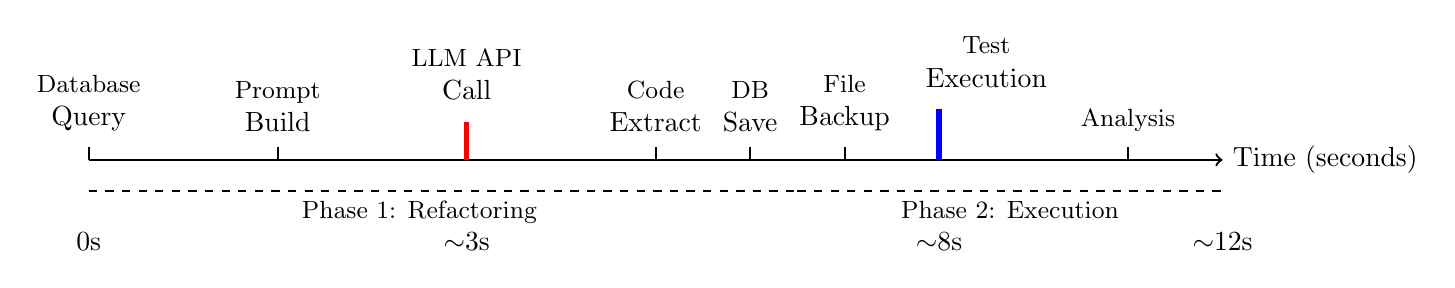
\begin{tikzpicture}[
    xscale=1.2,
    yscale=0.8
]

% Timeline
\draw[thick, ->] (0,0) -- (12,0) node[right] {Time (seconds)};

% Events
\node[above, align=center] at (0, 0.3) {\small Database\\Query};
\draw[thick] (0, 0) -- (0, 0.2);

\node[above, align=center] at (2, 0.3) {\small Prompt\\Build};
\draw[thick] (2, 0) -- (2, 0.2);

\node[above, align=center] at (4, 0.8) {\small LLM API\\Call};
\draw[thick, red, line width=2pt] (4, 0) -- (4, 0.6);

\node[above, align=center] at (6, 0.3) {\small Code\\Extract};
\draw[thick] (6, 0) -- (6, 0.2);

\node[above, align=center] at (7, 0.3) {\small DB\\Save};
\draw[thick] (7, 0) -- (7, 0.2);

\node[above, align=center] at (8, 0.3) {\small File\\Backup};
\draw[thick] (8, 0) -- (8, 0.2);

\node[above, align=center] at (9.5, 1.0) {\small Test\\Execution};
\draw[thick, blue, line width=2pt] (9, 0) -- (9, 0.8);

\node[above, align=center] at (11, 0.3) {\small Analysis};
\draw[thick] (11, 0) -- (11, 0.2);

% Phases
\draw[dashed, thick] (0, -0.5) -- (7.5, -0.5);
\node[below] at (3.5, -0.5) {\small Phase 1: Refactoring};

\draw[dashed, thick] (7.5, -0.5) -- (12, -0.5);
\node[below] at (9.75, -0.5) {\small Phase 2: Execution};

% Time markers
\node[below] at (0, -1) {0s};
\node[below] at (4, -1) {$\sim$3s};
\node[below] at (9, -1) {$\sim$8s};
\node[below] at (12, -1) {$\sim$12s};

\end{tikzpicture}
\caption{Typical Experiment Execution Timeline (Single Smell)}
\label{fig:timeline}
\end{figure}

\clearpage

\subsection{Research Questions Mapping}

\begin{figure}[h]
\centering
\begin{tikzpicture}[
    node distance=0.8cm,
    rq/.style={rectangle, draw, ultra thick, text width=8cm, text centered, minimum height=1cm, font=\small},
    metric/.style={rectangle, draw, text width=7cm, text centered, minimum height=0.7cm, font=\scriptsize, fill=blue!10},
]

\node[rq, fill=orange!20] (rq1) {\textbf{RQ1:} How effective are LLMs at refactoring test smells?};
\node[metric, below=0.3cm of rq1] (m1a) {Smell Removal Rate: $\frac{\text{smells removed}}{\text{total experiments}}$};
\node[metric, below=0.1cm of m1a] (m1b) {Test Preservation Rate: $\frac{\text{tests passing}}{\text{total experiments}}$};

\node[rq, fill=green!20, below=1cm of m1b] (rq2) {\textbf{RQ2:} Which prompt strategy performs best?};
\node[metric, below=0.3cm of rq2] (m2a) {Strategy Success: $\text{Compare}(\sigma_1, \sigma_2, \sigma_3)$};
\node[metric, below=0.1cm of m2a] (m2b) {Statistical Tests: ANOVA + post-hoc};

\node[rq, fill=yellow!20, below=1cm of m2b] (rq3) {\textbf{RQ3:} Which LLM model performs best?};
\node[metric, below=0.3cm of rq3] (m3a) {Model Success: $\text{Compare}(M_1, \ldots, M_6)$};
\node[metric, below=0.1cm of m3a] (m3b) {Cost Analysis: $\frac{\text{tokens used}}{\text{success rate}}$};

\node[rq, fill=purple!20, below=1cm of m3b] (rq4) {\textbf{RQ4:} Are there smell-specific patterns?};
\node[metric, below=0.3cm of rq4] (m4a) {Per-Smell Success Rates by Strategy/Model};
\node[metric, below=0.1cm of m4a] (m4b) {Interaction Effects: $\sigma \times M \times T$};

\end{tikzpicture}
\caption{Research Questions and Measurement Mapping}
\label{fig:research-questions}
\end{figure}

\end{document}
